\documentclass[a4paper,12pt]{article}
\usepackage[utf8]{inputenc}
\usepackage{amsmath}
\usepackage{comment}
\usepackage{graphicx}
\usepackage[left=1.5cm, right=1.5cm, top=2cm, bottom=2cm]{geometry}
\title{\textbf{COM 5120 Communication Theory}}
\author{\textbf{Midterm Make-up Exam}}
\date{November 17, 2022 \\ 
15:30 $\sim$ 17:20
}
\begin{document}
    \maketitle
    \textit{Note: }There are \textbf{6} problems with total 100 points within \textbf{3} pages, please write your answer with detail in the answer sheet.

    {\bf No credit without detail.  No calculator. Closed books.}

    \begin{enumerate}
    %%%%%%%%%%%%%%%%%%%%%%%%%%%%%%
        \item (25\%) 
            Consider the four waveforms shown in Figure 1. \\ 
            (a) Determine the dimensionality of the waveforms and a set of basis functions. \\
            (b)  Use the basis functions to represent the four waveforms by vectors $s_1$, $s_2$, $s_3$, and $s_4$. \\
            (c) Determine the minimum distance between any pair of vectors.
            \begin{figure}[h]
            	\centering
            	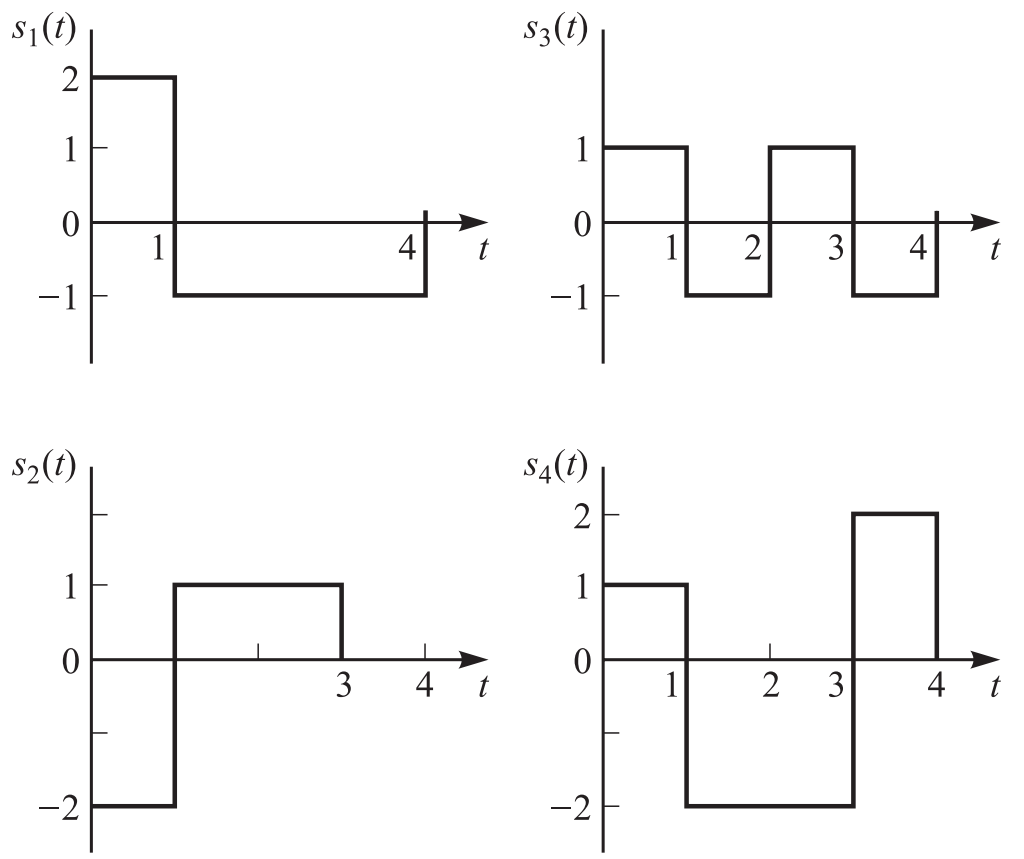
\includegraphics[scale=0.5]{Mid_fig5.png}
            	\caption{four waveforms $s_1(t)$, $s_2(t)$, $s_3(t)$, $s_4(t)$}
            % 	\label{fig}
            \end{figure}
    %%%%%%%%%%%%%%%%%%%%%%%%%%%%%%
        \item (25\%) 
            Suppose that $X$ is a Gaussian random variable with zero mean and unit variance. Let
            % Let $Y = aX^3 + b$, $a > 0$ 
            \begin{align*}
                Y = aX^3 + b, \;\; a > 0
            \end{align*}
            Determine and plot the PDF of $Y$. \\ 
    %%%%%%%%%%%%%%%%%%%%%%%%%%%%%%
        \item (10\%) 
            Consider the octal signal point constellations shown in Figure 2. \\ 
            (a) The nearest-neighbor signal points in the 8-QAM signal constellation are separated in distance by $A$ units. Determine the \textbf{radii} $a$ and $b$ of the inner and outer circles, respectively. \\
            (b) The adjacent signal points in the 8-PSK are separated by a distance of $A$ units. Determine the \textbf{radius} $r$ of the circle. \\
            % \begin{figure}[h]
            % 	\centering
            % 	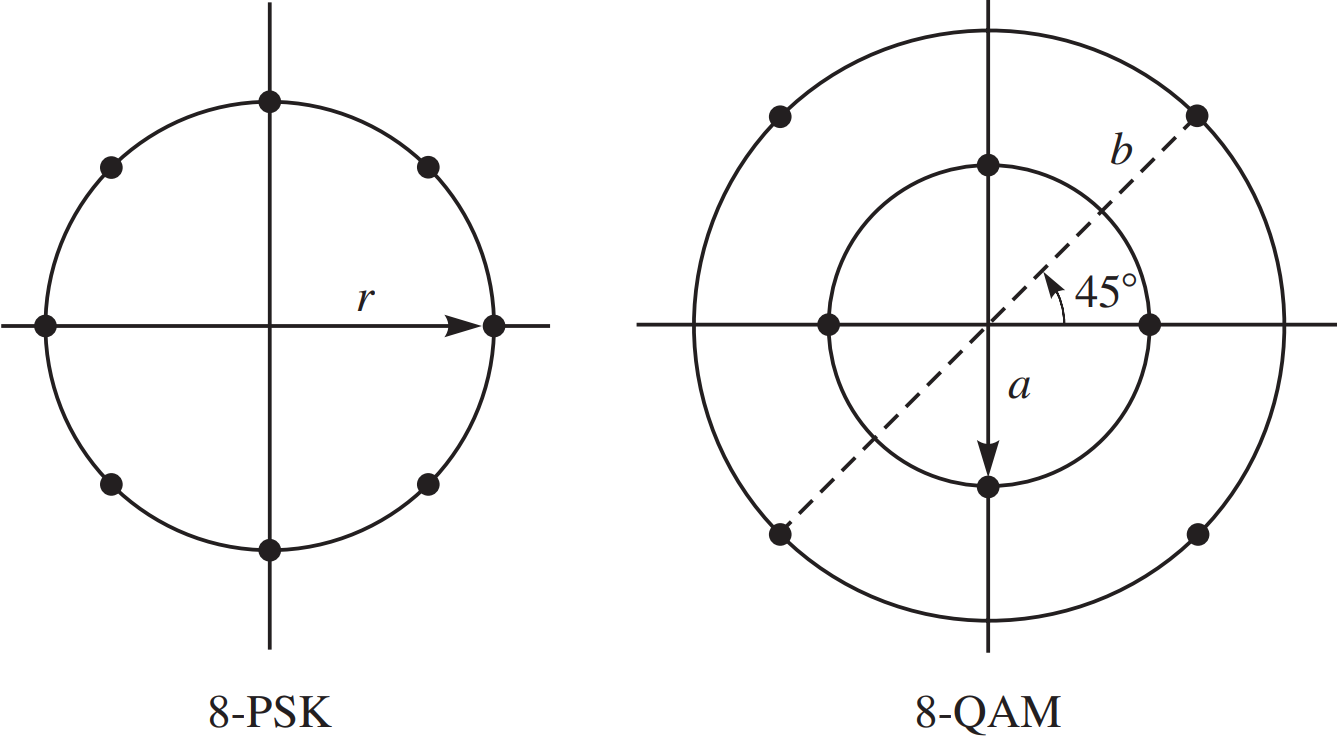
\includegraphics[scale=0.4]{Mid_fig2.png}
            % 	\caption{8-PSK and 8-QAM}
            % % 	\label{fig}
            % \end{figure}
            % \newpage
    %%%%%%%%%%%%%%%%%%%%%%%%%%%%%    
        \item (20\%) 
            Consider the 8-point QAM signal constellation shown in Figure 2. \\
            (a) Is it possible to assign 3 data bits to each point of the signal constellation such that the nearest (adjacent) points differ in only 1 bit position? \\ 
            (b) Determine the symbol rate if the desired bit rate is 90 Mbits/s. \\ 
            \begin{figure}[h]
            	\centering
            	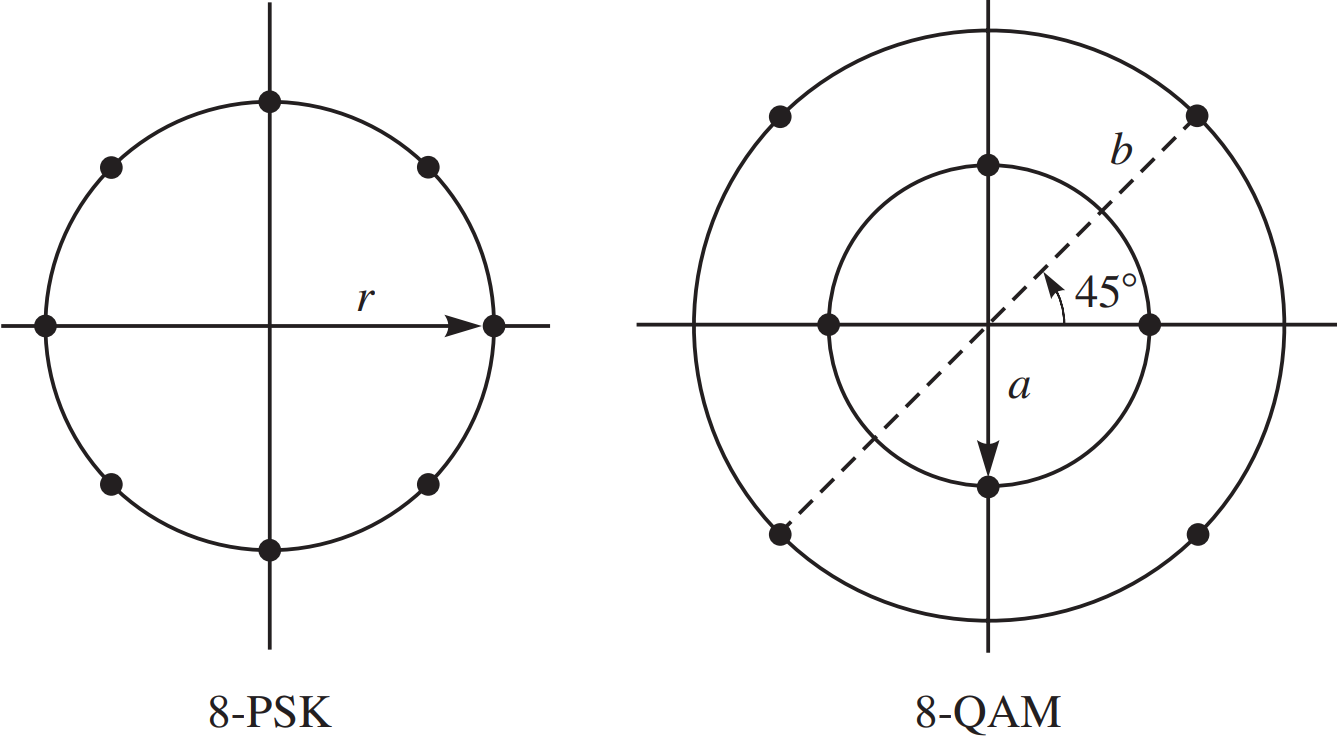
\includegraphics[scale=0.4]{Mid_fig2.png}
            	\caption{8-PSK and 8-QAM}
            % 	\label{fig}
            \end{figure}
    %%%%%%%%%%%%%%%%%%%%%%%%%%%%%%%%%%%%%%%%%%%%%%    
        \item (10\%) 
            A binary digital communication system employs the signals \\ 
            $$s_0(t) = 0, \; 0 \leq t \leq T$$
            $$s_1(t) = A, \; 0 \leq t \leq T$$
            for transmitting the information. This is called \emph{on-off signaling}. The demodulator crosscorrelates the received signal $r(t)$ with $s(t)$ and samples the output of the correlator at $t + T$. \\
            (a) Determine the \textbf{optimum detector} for an AWGN channel and the \textbf{optimum threshold}, assuming that the signals are equally probable. \\ 
            \textbf{Given that the correlation type demodulator employes a filter:} \\ 
            $$f(t) = \left\{ 
            \begin{aligned}
                \frac{1}{\sqrt{T}}, \; 0 \leq t < T \\
                 0, \; otherwise \\ 
            \end{aligned}
            \right.
            $$ \\
            (b) Determine the \textbf{probability of error} as a function of the SNR. How does on-off signaling compare with antipodal signaling? \\
    %%%%%%%%%%%%%%%%%%%%%%%%%%%%%%
        \item (10\%) 
            Consider the three waveforms $f_n(t)$ shown in Figure 3. \\ 
            (a) Show that these waveforms are \textbf{orthonormal}. \\ 
            (b) Express the waveform $x(t)$  as a \textbf{linear combination} of $f_n(t)$, $n = 1, 2, 3$ if 
            $$x = \left\{ 
            \begin{aligned}
                -2, \; 0 \leq t < 1 \\
                 6, \; 1 \leq t < 3 \\ 
                 4, \; 3 \leq t < 4 \\
            \end{aligned}
            \right.
            $$ \\
            and determine the \textbf{weighting coefficients}.
            \begin{figure}[h]
            	\centering
            	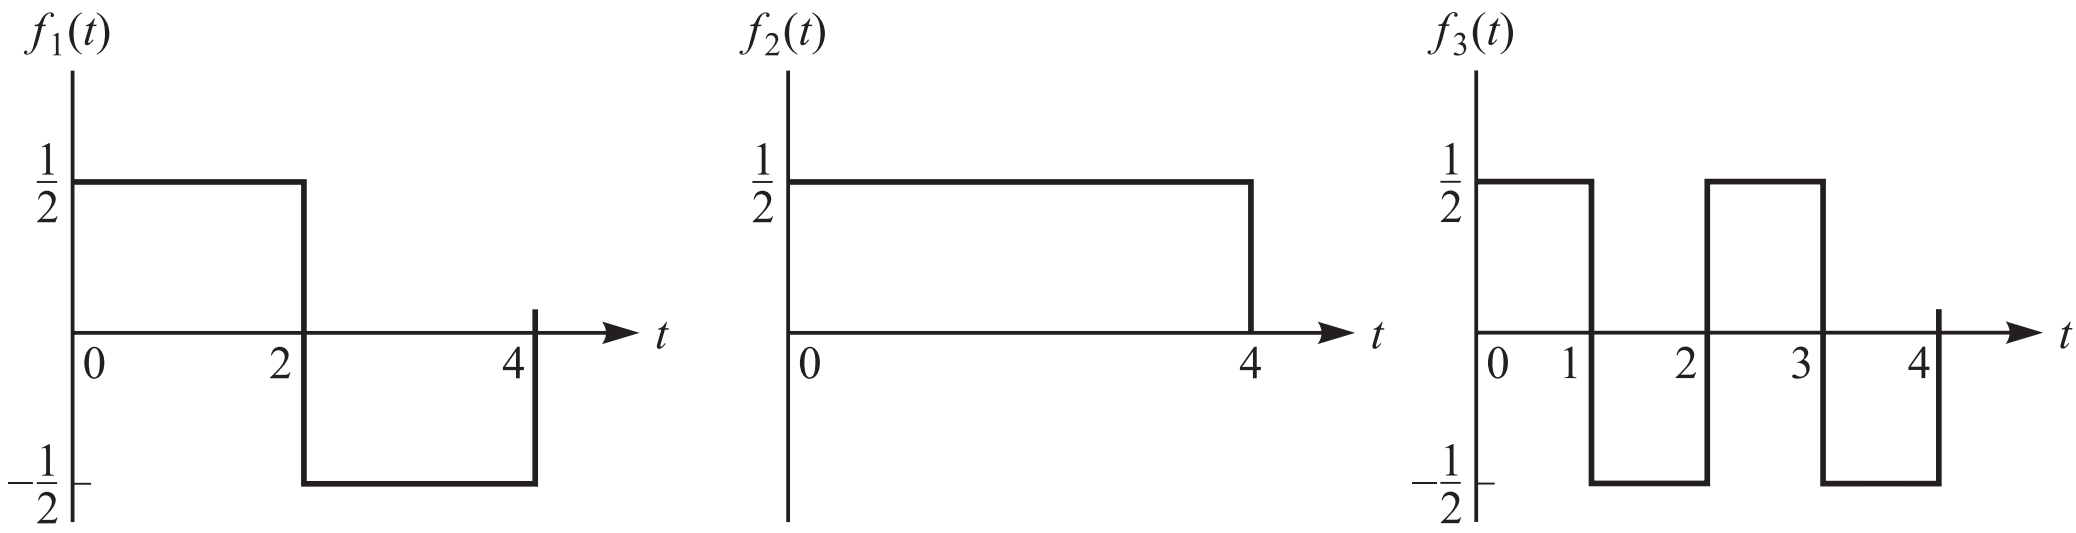
\includegraphics[scale=0.3]{Mid_fig1.png}
            	\caption{three waveforms $f_1(t)$, $f_2(t)$, $f_3(t)$}
            % 	\label{fig}
            \end{figure}
            % \newpage
    %%%%%%%%%%%%%%%%%%%%%%%%%%%%%%%%%%%%%%%%%%%%%%
    \end{enumerate}
    \rule{\textwidth}{0.4pt}
\end{document}


